\section[Proc Imágenes]{Procesamiento de Imágenes}
\begin{frame}\frametitle{Imágenes como funciones}
  \begin{itemize}
  \item Una imagen (en escala de grises) es una función $I(x,y)$ donde $x,y$ son variables discretas en coordenadas de imagen y la función $I$ es intensidad luminosa.
    \item Las imágenes también pueden considerarse como arreglos bidimensionales de números entre un mínimo y un máximo (usualmente 0-255).
    \item Aunque formalmente una imagen es un mapeo $f:\mathbb{R}^2\rightarrow \mathbb{R}$, en la práctica, tanto $x,y$ como $I$ son varialbes discretas con valores entre un mínimo y un máximo.
    \item Las imágenes de color son funciones vectoriales $f:\mathbb{R}^2\rightarrow \mathbb{R}^3$ donde cada componente de la función se llama canal.
%  \[I(x,y) = \left[\begin{tabular}{c}$r(x,y)$\\$g(x,y)$\\$b(x,y)$\end{tabular}\right]\]
  \end{itemize}
  \begin{figure}
    \centering
    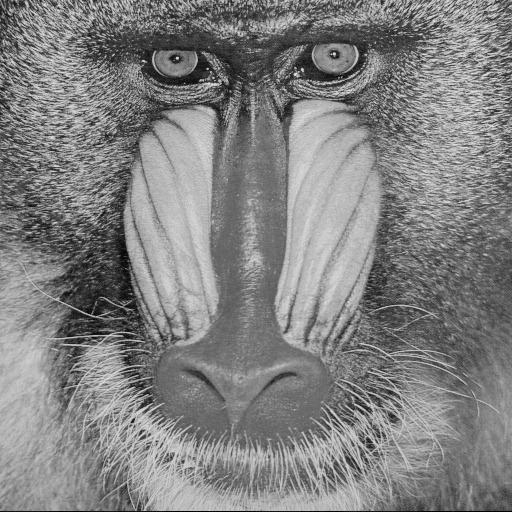
\includegraphics[width=0.3\textwidth]{Figures/baboon_grayscale.jpg}
    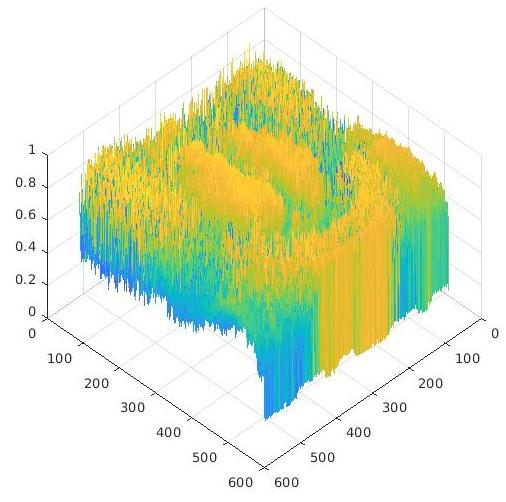
\includegraphics[width=0.35\textwidth]{Figures/BaboonPlot.jpg}
  \end{figure}
\end{frame}

\begin{frame}\frametitle{Operaciones básicas}
  Las operaciones básicas con una imagen son las mismas que con una señal cualquiera:
  \begin{itemize}
  \item Desfase
  \item Escalamiento
  \item Inversión en $x,y$
  \item Suma y Resta 
  \item Multiplicación
  \end{itemize}
  Ver ejercicios en Python.
\end{frame}

\begin{frame}\frametitle{Tipos de ruido}
  El ruido es una señal aleatoria $\eta(x,y)$, es decir, no sabemos cuánto vale para un punto determinado $(x,y)$ pero sí podemos caracterizarla.
  \[I_n(x,y) = I(x,y) + \eta(x,y)\]
  Existen varios tipos de ruido:
  \begin{itemize}
  \item Sal y pimienta: aleatoriamente aparecen puntos ya sea blancos o negros
  \item Ruido de impulso: aleatoriamente aparecen puntos blancos
  \item Ruido gausiano: $\eta(x,y)$ se distribuye 
  \end{itemize}
  Ver ejercicios en Python
\end{frame}

\begin{frame}\frametitle{SLID}
  Un sistema $S$ es un mapeo del conjunto de señales al conjunto de señales, es decir, es algo donde entra una señal $I(x,y)$ y sale otra señal $O(x,y)$:
  \[O(x,y) = S[I(x,y)]\]
  Los sistemas lineales invariantes ante el desfase son sistemas en los que se cumplen las siguientes propiedades:
  \begin{itemize}
  \item \textbf{Aditividad y homogeneidad:}
    \[S[\alpha I_1(x,y) + \beta I_2(x,y)] = \alpha S[I_1(x,y)] + \beta S[I_2(x,y)]\]
  \item \textbf{Invarianza ante el desfase:}
    \[\textrm{Si} \qquad S[I(x,y)] = O(x,y) \qquad\textrm{entonces:}\]
    \[S[I(x-i, y-j)] = O(x-i, y-j) \qquad \forall i,j \in \mathbb{Z}\]
  \end{itemize}
  Los SLID se pueden caracterizar de varias formas:
  \begin{itemize}
  \item Ecuaciones en diferencias
  \item Funciones de transferencia
  \item Respuesta al impulso
  \end{itemize}
\end{frame}

\begin{frame}\frametitle{Convolución}
  Si se conoce la respuesta al impulso $H(x,y)$ de un sistema SLID, se puede obtener la salida $O(x,y)$ ante cualquier entrada $I(x,y)$, mediante la convolución, definida como:
  \[O(x,y) = I(x,y)*H(x,y) = \sum_{i=-\infty}^\infty \sum_{j=-\infty}^\infty I(i,j)H(x-i, y-j)\]
  Ejemplos:
  \[\left[\begin{tabular}{cccc}
      3 & 1 & 4 & 1\\
      5 & 9 & 2 & 6\\
      5 & 3 & 5 & 8\\
      9 & 7 & 9 &3
    \end{tabular}\right]* [1\quad -1] =
  \left[\begin{tabular}{ccccc}
      3 & -2 & 3 & -3 & -1\\
      5 & 4 & -7 & 4 & -6\\
      5 & -2 & 2 & 3 & -8\\
      9 & -2 & 2 & -6 & -3
    \end{tabular}\right]\]

  \[\left[\begin{tabular}{cccc}
      3 & 1 & 4 & 1\\
      5 & 9 & 2 & 6\\
      5 & 3 & 5 & 8\\
      9 & 7 & 9 &3
    \end{tabular}\right]* \left[\begin{tabular}{c}1 \\ -1\end{tabular}\right] =
  \left[\begin{tabular}{cccc}
      3 & 1 & 4 & 1\\
      2 & 8 & -2 & 5\\
      0 & -6 & 3 & 2\\
      4 & 4 & 4 & -5\\
      -9 & -7 & -9 & -3
    \end{tabular}\right]\]
\end{frame}

\begin{frame}\frametitle{Manejo de bordes}
  En el ejemplo anterior, supusimos que fuera de la matriz, todos los elementos son cero. Sin embargo existen otras formas de manejar los borde:
  \begin{itemize}
  \item Recortar: suponer que fuera de la matriz los valores son cero. En el caso de una imagen, suponemos pixeles negros fuera de la imagen.
  \item Wrap around: suponer que la imagen es periódica.
  \item Borde repetido: suponer que los valores de los bordes se mantienen iguales fuera de la imagen.
  \item Reflexión: fuera de los bordes se tiene una imagen en espejo.
  \end{itemize}
\end{frame}

\begin{frame}\frametitle{Propiedades de la convolución}
  \begin{itemize}
  \item Es conmutativa: $H*I = I*H$
  \item Es asociativa: $H*I_1*I_2$ = $H*(I_1*I_2)$ = $(H*I_1)*I_2$
  \item Es distributiva: $H*(I_1 + I_2) = H*I_1 + H*I_2$
  \item Es lineal: $H*(\alpha I_1 + \beta I_2) = \alpha H*I_1 + \beta H*I_2$
  \end{itemize}
  En el caso de secuencias finitas bidimensionales:
  \begin{itemize}
  \item Si $I\in\mathbb{R}^{r_1\times c_1}$ y $H\in\mathbb{R}^{r_2\times c_2}$, entonces $(I*H) \in \mathbb{R}^{(r_1+r_2-1)\times (c_1 + c_2 - 1)}$
  \item Si $I\in\mathbb{R}^{r_1\times c_1}$ y $H\in\mathbb{R}^{r_2\times c_2}$, la complejidad de la convolución es del orden de $r_1 r_2 c_1 c_2$
  \end{itemize}
\end{frame}

\begin{frame}\frametitle{Conexión de sistemas SLID}
  Dos o más SLID se pueden conectar de dos formas distintas:
  \begin{itemize}
  \item Conexión en paralelo:
    \begin{figure}
      \centering
      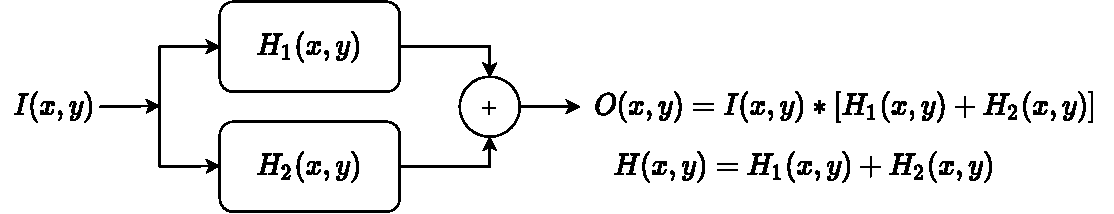
\includegraphics[scale=0.7]{Figures/Parallel.pdf}
    \end{figure}
  \item Conexión en cascada:
    \begin{figure}
      \centering
      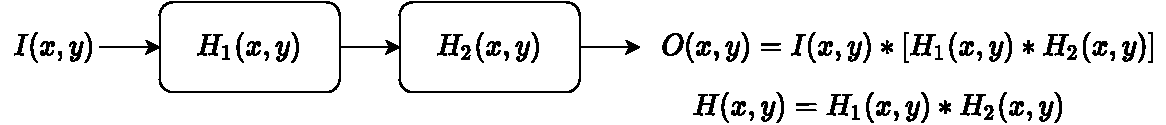
\includegraphics[scale=0.7]{Figures/Cascade.pdf}
    \end{figure}
  \end{itemize}
\end{frame}

\begin{frame}\frametitle{Gradiente}
  El gradiente de una imagen está definido como:
  \[\nabla I = \left[\frac{\partial I}{\partial x}, \frac{\partial I}{\partial y}\right]\]
  Las derivadas parciales se puede aproximar mediante diferencias finitas:
  \begin{eqnarray*}
    \frac{\partial I}{\partial x} &=& \lim_{\Delta x \rightarrow 0}\frac{I(x + \Delta x, y) - I(x,y)}{\Delta x}\approx I_{i,j} - I_{i,j-1}\\
    \frac{\partial I}{\partial y} &=& \lim_{\Delta y \rightarrow 0}\frac{I(x, y + \Delta y) - I(x,y)}{\Delta y}\approx I_{i,j} - I_{i-i,j}
  \end{eqnarray*}
  donde $(i,j)$ representan las coordenadas de imagen renglón-columna. Estas diferencias finitas se puede obtener mediante una convolución:
  \begin{eqnarray*}
    \frac{\partial I}{\partial x} &\approx& I * [1\quad -1]\\
    \frac{\partial I}{\partial y} &\approx& I * \left[\begin{tabular}{c}1\\-1\end{tabular}\right]
  \end{eqnarray*}
\end{frame}

\begin{frame}\frametitle{Gradiente}
  Una mejor aproximación de la derivada es no solo tomar la diferencia entre el valor actual y el anterior $(I_{i,j} - I_{i-1,j})$, sino promediarlo con la diferencia $(I_{i+1,j} - I_{i,j})$:
  \[\frac{1}{2}[(I_{i,j} - I_{i-1,j}) + (I_{i+1,j} - I_{i,j})] = \frac{1}{2}(I_{i+1,j} - I_{i-1,j})\]
  Generalmente se ignora el coeficiente y se utilizan los siguientes Kernels:
  \begin{eqnarray*}
    \frac{\partial I}{\partial x} &\approx& I * [1\quad 0\quad -1]\\
    \frac{\partial I}{\partial y} &\approx& I * \left[\begin{tabular}{c}1\\ 0\\-1\end{tabular}\right]
  \end{eqnarray*}
\end{frame}

\begin{frame}\frametitle{El filtro de Sobel}
  El Operador de Sobel o Filtro de Sobel consiste en un Kernel que permite obtener las derivadas parciales, aproximadas por diferencias finitas, y promediadas con un filtro Gaussiano:
  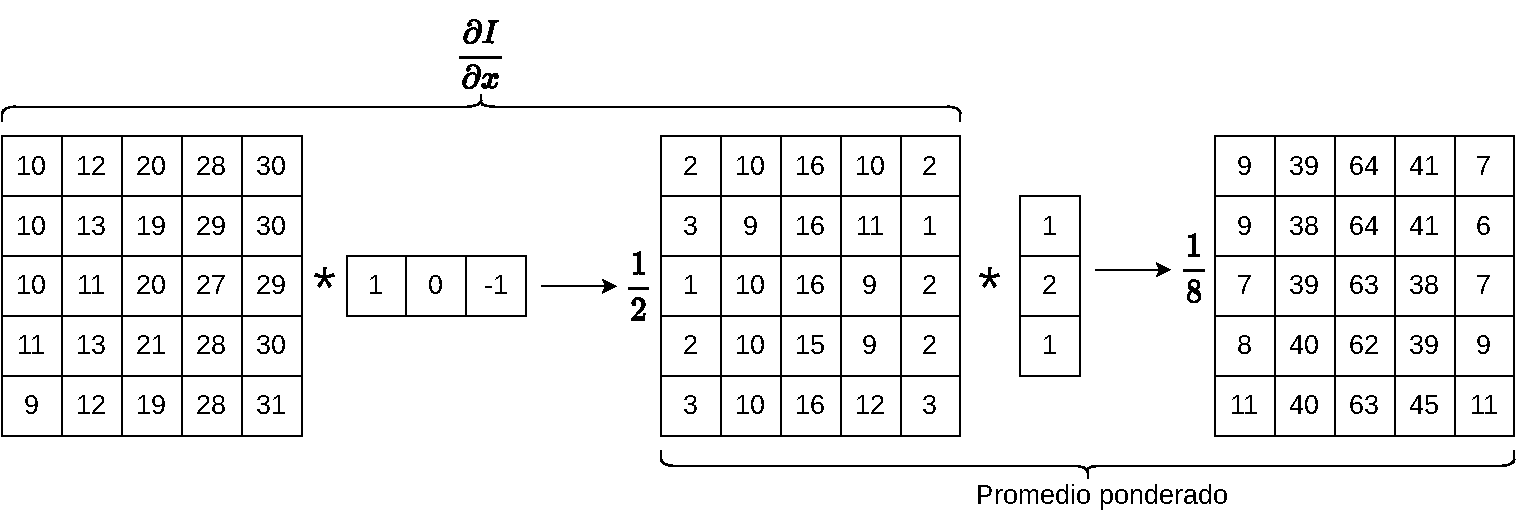
\includegraphics[width=\textwidth]{Figures/SobelX1.pdf}
  Se realiza un proceso similar para la derivada parcial en $Y$. Aplicando la propiedad asociativa de la convolución, se obtienen los siguientes ekernels:
  \[S_x = \left[\begin{tabular}{ccc}1 & 0 & -1\\2 & 0 & -2\\1 & 0 & -1 \end{tabular}\right]\qquad\qquad
  S_y = \left[\begin{tabular}{ccc}1 & 2 & 1\\0 & 0 & 0\\-1 & -2 & -1 \end{tabular}\right]\]
\end{frame}

\begin{frame}\frametitle{Ejemplo}
\end{frame}

\begin{frame}\frametitle{Magnitud y Ángulo}
  El gradiente en cada pixel de la imagen se puede calcular mediante la approximación de las derivadas parciales:
  \begin{eqnarray*}
    \frac{\partial I}{\partial x} &\approx& I * Sx = G_x\\
    \frac{\partial I}{\partial y} &\approx& I * Sy = G_y\\
  \end{eqnarray*}
  En la mayoría de las aplicaciones es más últil expresar el gradiente en forma polar:
  \[ \nabla I = G_m \angle G_a \]
  Donde la magnitud del gradiente y la fase, para cada pixel, se calculan como:
  \begin{eqnarray*}
    G_{m_{i,j}} &=& \sqrt{G_{x_{i,j}}^2 + G_{y_{i,j}}^2}\\
    G_{a_{i,j}} &=& \atantwo(G_{y_{i,j}}, G_{y_{i,j}})\\
  \end{eqnarray*}
\end{frame}

\begin{frame}\frametitle{Detector de Bordes de Canny}
  El detector de bordes de Canny es un detector basado en gradiente que consta de los siguientes pasos básicos:
  \begin{enumerate}
  \item Obtención del gradiente en magnitud y ángulo, mediante operadores de Sobel
  \item Supresión de puntos no máximos
  \item Aplicación de un doble umbral
  \end{enumerate}
  Aunque no es un paso en sí del Detector de Canny, generalmente se considera como primer paso la aplicación de un filtro Gaussiano para disminuir el ruido. 
\end{frame}

\begin{frame}\frametitle{Obtención del gradiente}
  Después del filtro Gaussiano, el primer paso es obtener el gradiente de la imagen mediante el Filtro de Sobel, en la forma de magnitud y ángulo:\\
  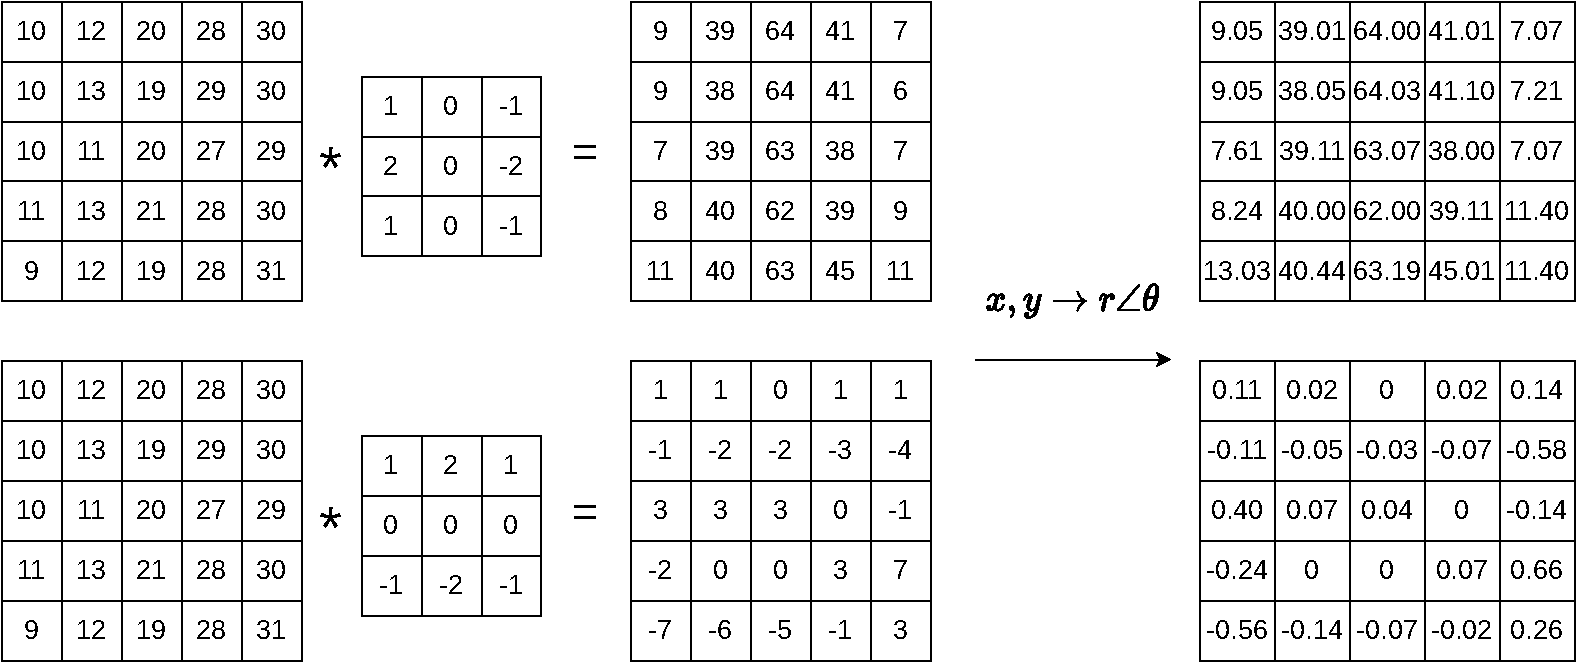
\includegraphics[width=0.9\textwidth]{Figures/SobelXY.pdf}
\end{frame}

\begin{frame}\frametitle{Supresión de no máximos}
  Este paso consiste en comparar la magnitud de cada pixel, con los pixeles anterior y posterior en la dirección del gradiente.
  Aunque la fase es un ángulo en $[-\pi, \pi]$, la dirección del gradiente se debe redondear a algún valor correspondiente a la connectividad 8: \textit{N, NE, E, SE}. Debido a que el pixel se compara en la dirección positiva y negativa del gradiente, no es necesario considerar las direcciones \textit{S, SW, W, NW}.
  \begin{figure}
    \centering
    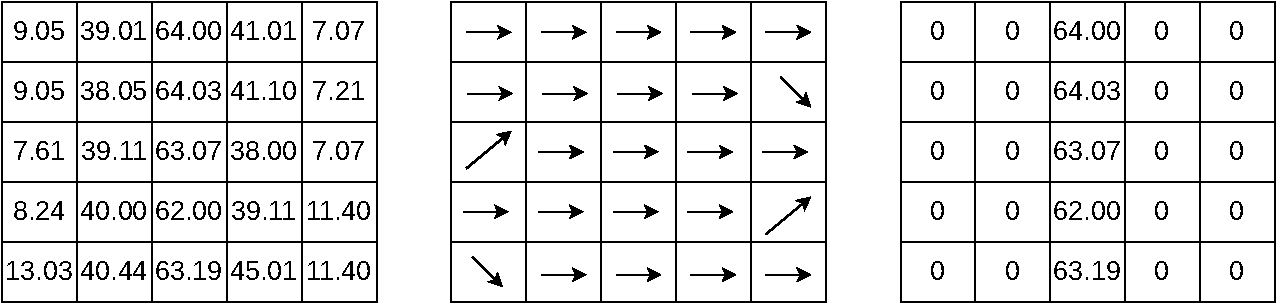
\includegraphics[width=0.9\textwidth]{Figures/SobelMA.pdf}
  \end{figure}
  Para cada pixel $p_i$, considere $p_{i+1}$, el pixel siguiente en la dirección del gradiente, y $p_{i-1}$, el pixel anterior, en la dirección del gradiente. El valor para cada pixel $q_i$ en la imagen resultante es:
  
  \[q_i = \begin{cases}p_i\qquad\qquad\textrm{si}\qquad p_i > p_{i+1} \qquad\textrm{y}\qquad p_i > p_{i-1}\\
  0\qquad\qquad\textrm{en otro caso}\end{cases}\]
\end{frame}

\begin{frame}\frametitle{Aplicación de doble umbral}
  En este paso, se definen dos umbrales: superior $\theta_u$ e inferior $\theta_l$. Los pixeles se clasifican en tres tipos:
  \begin{itemize}
  \item Fuertes: pixeles con magnitud del gradiente mayor que el umbral superior $|\nabla | > \theta_u$
  \item Débiles: pixeles con magnitud del gradiente entre ambos umbrales $\theta_l < |\nabla| < \theta_u$
  \item Suprimidos: pixeles con magnitud del gradiente menor que el umbral inferior $|\nabla| < \theta_l$
  \end{itemize}
  La imagen resultante se forma con las siguientes reglas:
  \begin{itemize}
  \item Todos los pixeles fuertes son parte de un borde.
  \item Todos los pixeles suprimidos no son bordes. 
  \item Los pixeles débiles son parte de un borde solo si están conectados (en conectividad 8) con un pixel fuerte.
  \end{itemize}
  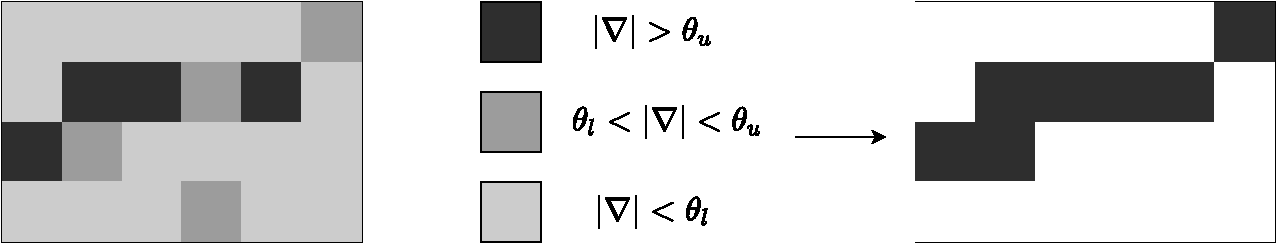
\includegraphics[width=\textwidth]{Figures/DoubleThreshold.pdf}
\end{frame}

\begin{frame}\frametitle{Espacios de color}
En las imágenes el color se representa mediante la combinación de 3 valores (generalmente, 3 bytes). Las diferentes formas de representar el color mediante estos tres valores se conocen como \textit{espacios de color}.
\end{frame}
